\section{Deferred tables and figures}
\label{app:floats}

This appendix collects tables and figures deferred from the main text for space.
All numbers are referenced from, and discussed in, the sections indicated.

\ificlrcompact\AlgCompSel\TabPredictor\fi

\subsection{Alignment across sizes (\S\ref{sec:representations})}
\label{app:align}

\begin{figure}[h]
\centering
% source: results/m2_cka/*/cka_heatmap.png and results/m2_maps/*/maps_r2.png
% (gitignored, regenerable at paper quality; dashed reference lines per style guide)
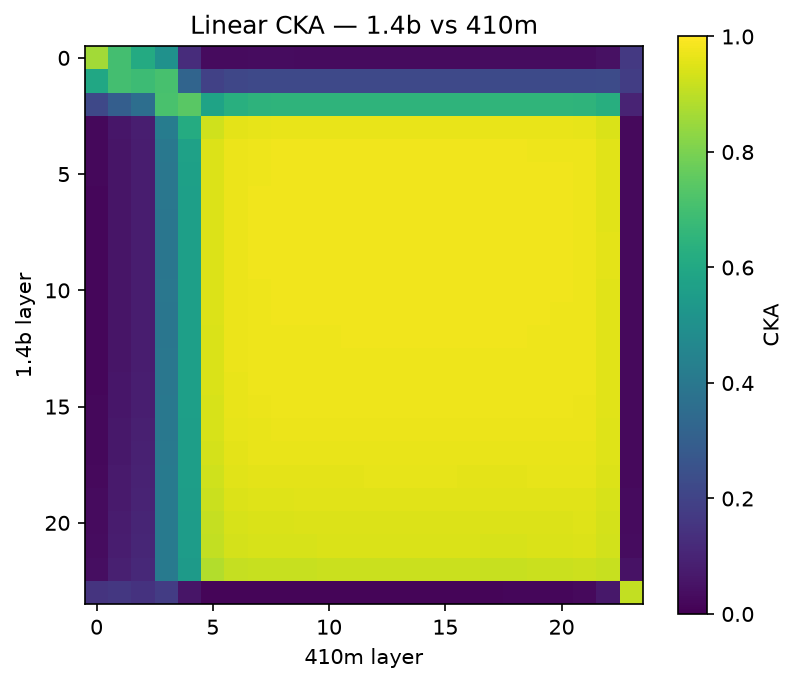
\includegraphics[width=0.46\linewidth]{figures/cka_heatmap.png}
\hfill
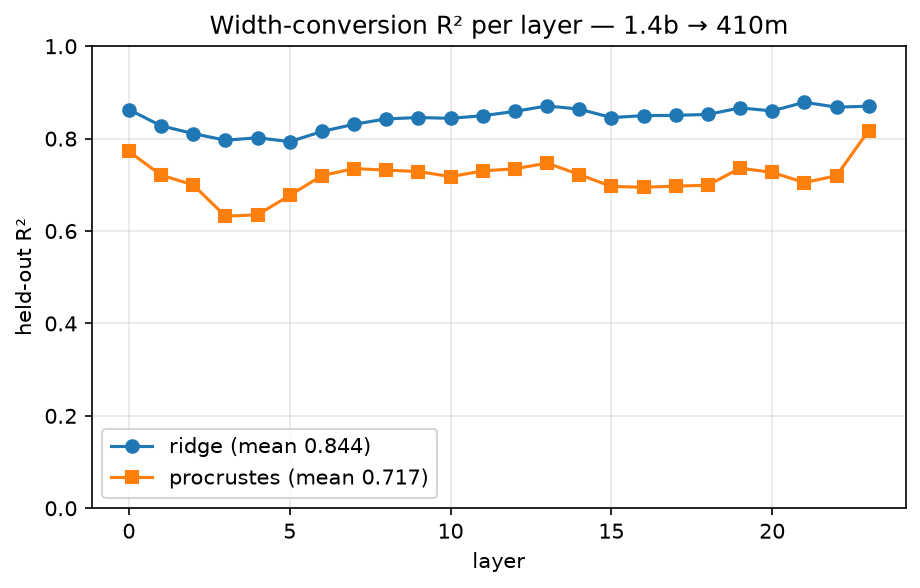
\includegraphics[width=0.46\linewidth]{figures/maps_r2.png}
\caption{Alignment across sizes for the primary pair (1.4B$\,\to\,$410M).
\textbf{(left)} Linear CKA between all $24\times24$ layer pairs: a saturated
middle band (layers $\sim$4--22 mutually $\approx1.0$) confirms coarse
correspondence but resolves no sharp per-layer match. \textbf{(right)} Held-out
$R^2$ of the per-layer activation maps: ridge (full linear) and Procrustes
(rotation$+$scale) track each other and dip together at layers 3--5, the layers
CKA also flags as distinct.}
\label{fig:align}
\end{figure}

\begin{table}[h]
\centering
\caption{Alignment across sizes, held-out. Activations align strongly under a
linear map; raw parameters, even in the cleanest (embedding) case, do not.
Best (highest) map per row in \textbf{bold}.}
\label{tab:align}
\begin{tabular}{lccc}
\toprule
Target & CKA & Ridge $R^2$ & Procrustes $R^2$ \\
\midrule
Pooled activations (per-layer mean) & $0.883^{\dagger}$ & \textbf{0.844} & 0.717 \\
\midrule
Input embedding & 0.512 & \textbf{0.248} & 0.167 \\
Output embedding (unembedding) & 0.678 & \textbf{0.386} & 0.242 \\
\bottomrule
\end{tabular}
\\[3pt]
{\footnotesize $^{\dagger}$ For activations, the diagonal mean of the
$24\times24$ linear-CKA matrix, which saturates in the middle band
(Figure~\ref{fig:align}, left); for embeddings, linear CKA before mapping.}
\end{table}

\subsection{Projection diagnostics (\S\ref{sec:projection})}
\label{app:projection}

\begin{table}[h]
\small
\begin{minipage}[t]{0.55\linewidth}
\centering
\caption{Relative Frobenius error of projected weights vs.\ the actual 410M
weights (mean over 24 layers). Every target-free error exceeds $1$ (worse than
zero); lower per row in \textbf{bold}.}
\label{tab:proj}
\setlength{\tabcolsep}{4pt}
\begin{tabular}{lcc}
\toprule
Weight & Projection & Operator$^{\dagger}$ \\
       & (target-free) & (fitted) \\
\midrule
$Q$            & 1.471 & \textbf{0.658} \\
$K$            & 1.591 & \textbf{0.758} \\
$V$            & 1.390 & \textbf{0.804} \\
$O$            & 1.724 & \textbf{0.795} \\
\texttt{MLP\_UP}   & 1.668 & \textbf{0.683} \\
\texttt{MLP\_DOWN} & 1.723 & \textbf{0.686} \\
\bottomrule
\end{tabular}
\\[3pt]
{\footnotesize $^{\dagger}$ A single $(A,B)$ shared across layers per type; it
peeks at the target and so upper-bounds the linearly explainable fraction. A
\emph{per-layer} fit is degenerate (error $\to 0$ around any full-rank $W$) and
is not reported.}
\end{minipage}\hfill
\begin{minipage}[t]{0.43\linewidth}
\centering
\caption{Zero-shot dense-projected quality (strided WikiText-103 perplexity);
the projected model does not beat random init. Best (lowest) in \textbf{bold}.}
\label{tab:anchor}
\begin{tabular}{lc}
\toprule
Model & Perplexity \\
\midrule
real 1.4B (reference)        & \textbf{11.5} \\
real 410M (upper anchor)     & 15.6 \\
random-init 410M (lower)     & 65{,}962 \\
\midrule
proj., LN from 410M   & 181{,}242 \\
proj., LN from 1.4B & $10^{13}$ \\
\bottomrule
\end{tabular}
\\[3pt]
{\footnotesize With fresh \emph{neutral} LayerNorms (gain 1, bias 0) the same
projected matrices score $\sim$12.3k quick-perplexity --- $\sim$15$\times$ better
than the 181{,}242 row and $\sim$5$\times$ better than random init --- so much of
the collapse is LayerNorm mismatch, not weight destruction alone
(\S\ref{sec:race}); the structure-mixing diagnosis still holds directionally.}
\end{minipage}
\end{table}

\subsection{Spectral residual test (\S\ref{sec:residuals})}
\label{app:spectral}

\begin{table}[h]
\centering
\caption{Test 1 (spectral). Effective rank of the residual $\Delta$ vs.\ a
per-type shuffled control and a shape/scale-matched Gaussian control. $\Delta$
sits $2.8$--$6.4\%$ below both in every type --- a faint, non-isotropic
concentration, not a learnable direction.}
\label{tab:erank}
\begin{tabular}{lccc}
\toprule
Weight & $\Delta$ erank & Shuffled & Gaussian \\
\midrule
$Q$            & 771.3 & 824.1 & 824.1 \\
$K$            & 784.0 & 824.0 & 824.1 \\
$V$            & 801.2 & 824.2 & 824.1 \\
$O$            & 792.2 & 824.1 & 824.1 \\
\texttt{MLP\_UP}   & 947.2 & 989.4 & 989.4 \\
\texttt{MLP\_DOWN} & 934.8 & 989.4 & 989.4 \\
\bottomrule
\end{tabular}
\end{table}

\begin{figure}[h]
\centering
% source: results/m4_residuals/*/delta_spectra.png (gitignored, regenerable)
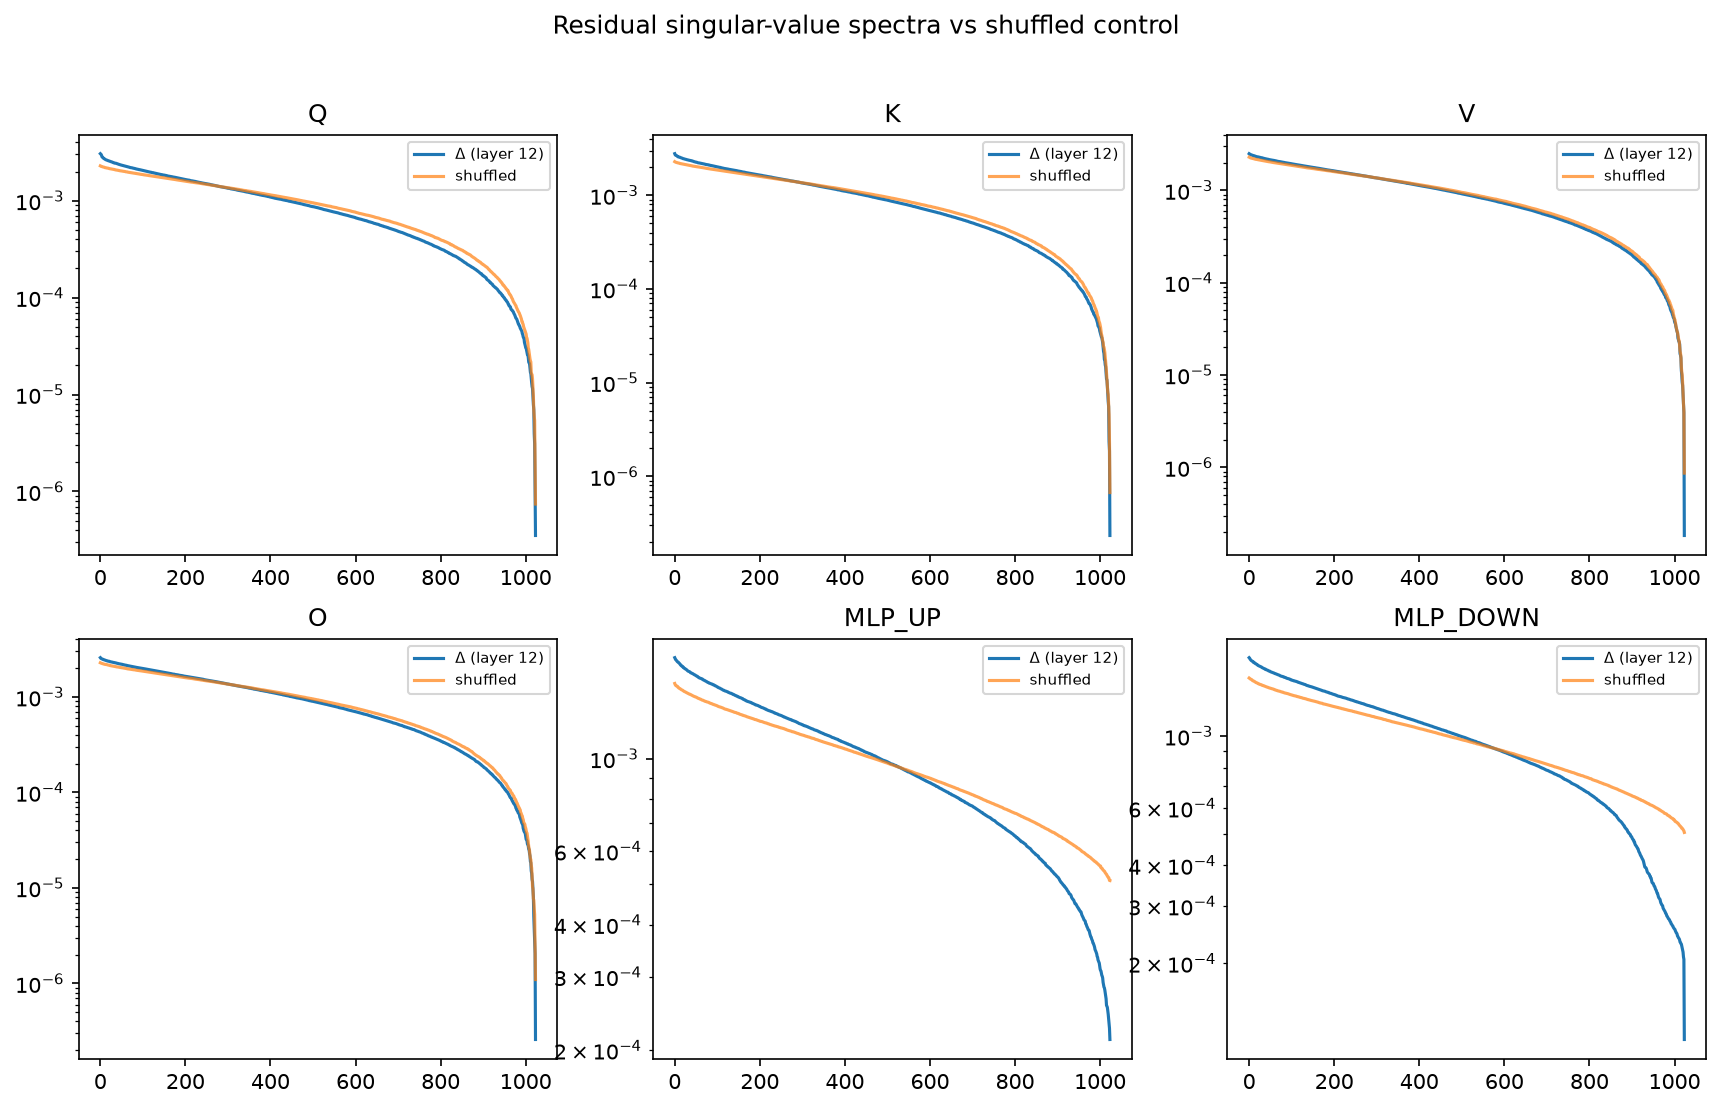
\includegraphics[width=0.6\linewidth]{figures/delta_spectra.png}
\caption{Test 1 (spectral). Singular-value spectrum of the residual $\Delta$
against shuffled and Gaussian controls. $\Delta$ concentrates $2.8$--$6.4\%$ more
than either control in every weight type --- a faint, generic non-isotropy that
carries no layer-specific, predictable signal (Table~\ref{tab:predictor}).}
\label{fig:spectra}
\end{figure}

\subsection{Extended evaluation, primary pair (\S\ref{sec:race:hardening})}
\label{app:extended}

\begin{table}[h]
\centering
\caption{Extended evaluation of the 30M primary-pair checkpoints and the
real-410M reference. Guess floors: arc\_easy $0.25$, hellaswag $0.25$, piqa
$0.50$, lambada $\approx0$ (open-vocabulary). Best converted arm in
\textbf{bold}; the ordering holds on all six metrics. Single-seed checkpoints.
This table predates the rescale-lever ablation and reports the compensation
contrast (\textsc{hybrid} vs.\ \textsc{subclone}); the rescale gains of
Tables~\ref{tab:ladder}--\ref{tab:seeded} stack on top of it.}
\label{tab:extended}
\begin{tabular}{lrrrrrr}
\toprule
Model & C4 ppl & wk@2048 & lambada & arc\_easy & hellaswag & piqa \\
\midrule
\textbf{hybrid} & \textbf{90.7} & \textbf{109.8} & \textbf{0.076} & \textbf{0.313} & \textbf{0.266} & \textbf{0.555} \\
subclone        & 162.7 & 346.3 & 0.005 & 0.308 & 0.263 & 0.548 \\
projection      & 380.5 & 1{,}210 & 0.000 & 0.272 & 0.258 & 0.539 \\
random          & 518.8 & 1{,}788 & 0.000 & 0.264 & 0.256 & 0.532 \\
\midrule
real 410M       & 21.0 & 14.5 & 0.516 & 0.519 & 0.337 & 0.667 \\
\bottomrule
\end{tabular}
\end{table}

\subsection{Primary-pair seeded verdict (\S\ref{sec:race:seeded})}
\label{app:seeded}

\begin{table}[h]
\centering
\footnotesize
\caption{Primary-pair final WikiText-103 perplexity across three data-draw seeds
(30M tokens; identical budget/schedule per seed). \textsc{hybrid\_rs} wins every
paired comparison; its worst seed beats \textsc{subclone\_rs}'s best.}
\label{tab:seeded}
\begin{tabular}{lrrrr}
\toprule
Init & seed 0 & seed 1 & seed 2 & mean $\pm$ std \\
\midrule
subclone\_rs        & 86.4 & 93.7 & 88.9 & $89.7 \pm 3.7$ \\
\textbf{hybrid\_rs} & \textbf{83.0} & \textbf{86.0} & \textbf{82.8} & $\mathbf{84.0 \pm 1.8}$ \\
\bottomrule
\end{tabular}
\end{table}

\subsection{Held-out pair per-seed detail (\S\ref{sec:race:hardening})}
\label{app:unseen}

\begin{table}[h]
\centering
\caption{Held-out pair (410M$\to$160M), final WikiText-103 perplexity across
three data-draw seeds (30M tokens). Transfer beats from scratch $\sim$$13\times$
on every seed; hybrid and subclone are a statistical tie on this
depth-dominated pair (overlapping $\pm1\sigma$).}
\label{tab:unseen}
\begin{tabular}{lrrrr}
\toprule
Init & seed 0 & seed 1 & seed 2 & mean $\pm$ std \\
\midrule
\textbf{hybrid} & 117.5 & 113.6 & 108.5 & $\mathbf{113.2 \pm 4.5}$ \\
subclone        & 115.0 & 121.6 & 118.9 & $118.5 \pm 3.3$ \\
random          & 1{,}464.4 & 1{,}571.5 & 1{,}479.6 & $1{,}505.2 \pm 57.9$ \\
\bottomrule
\end{tabular}
\end{table}

\paragraph{Metric robustness (held-out pair).}
\label{app:unseen-metrics}
On the held-out 410M$\to$160M pair the hybrid-vs-subclone tie holds on every
metric beyond WikiText-103: C4 perplexity $91.1$ vs.\ $94.2$, perplexity at
$2\times$ context $111.8$ vs.\ $110.2$, LAMBADA $11.0\%$ vs.\ $10.7\%$ (others
within noise), while random sits at C4 $514$ and LAMBADA $0$; the real-160M
anchor (LAMBADA $35.4\%$) matches published Pythia numbers. These cells are
single-seed.

\begin{figure}[h]
\centering
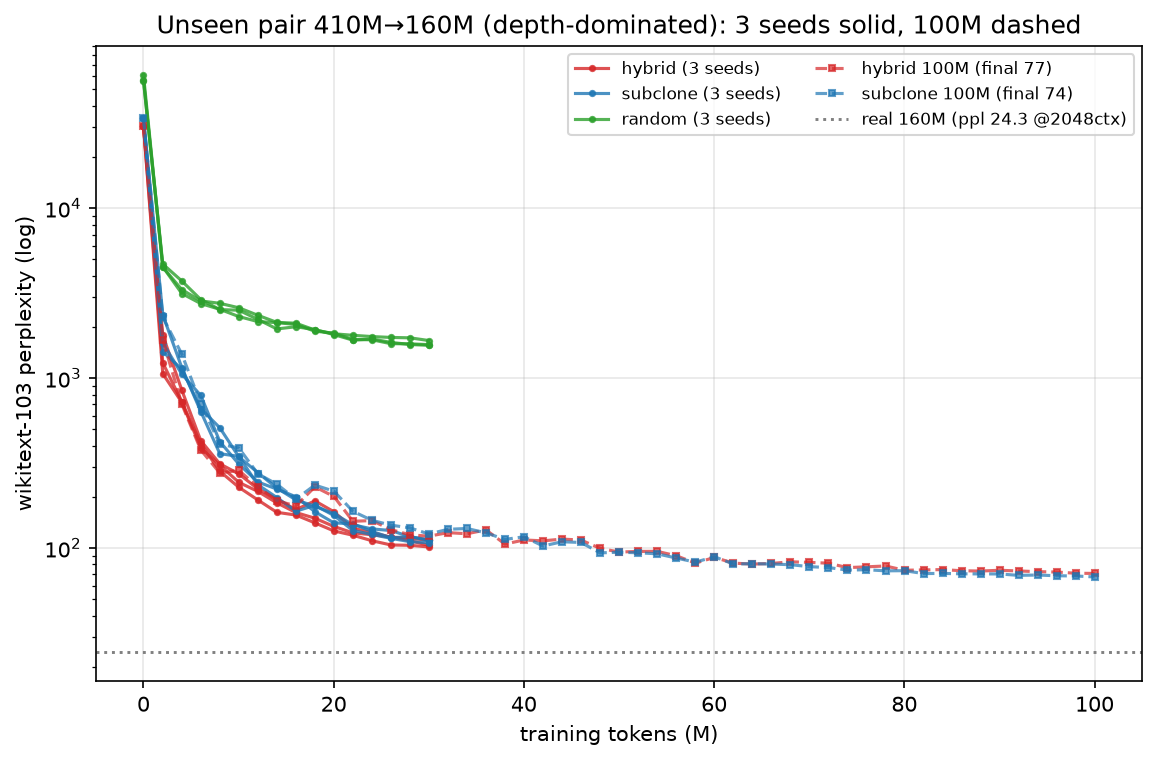
\includegraphics[width=0.92\linewidth]{figures/m5b_curves.png}
\caption{\textbf{Held-out pair (410M$\to$160M), three seeds.} Full WikiText-103
perplexity (log scale) versus tokens; bands span the three data-draw seeds and
the dashed line marks the real Pythia-160M reference. Transfer inits (hybrid,
subclone) sit an order of magnitude below random throughout and overlap each
other --- the depth-dominated regime where compensation's width-repair edge is
neutral (Table~\ref{tab:unseen}), yet the $\sim$$13\times$ margin over from
scratch is preserved on every seed.}
\label{fig:m5bcurves}
\end{figure}

\subsection{Scale pair (\S\ref{sec:race:scale})}
\label{app:scale}

\begin{table}[h]
\centering
\caption{Scale pair (6.9B$\to$1.4B), 30M tokens, single seed. The two levers that
stack at smaller scale here \emph{anti}-synergize --- each alone beats the
combination --- though every transfer arm still beats from scratch
(\S\ref{sec:race:scale}).}
\label{tab:scale}
\begin{tabular}{llr}
\toprule
Init & Construction & Final ppl (30M) \\
\midrule
random       & from scratch             & 1{,}413 \\
hybrid\_rs   & compensation $+$ rescale & 1{,}213 \\
hybrid       & compensation only        & 776 \\
subclone\_rs & rescale only             & \textbf{572} \\
\bottomrule
\end{tabular}
\end{table}

\section{Deferred discussion}
\label{app:discussion}

\subsection{An honest correction (\S\ref{sec:race:seeded})}
\label{app:correction}

The rescale lever corrects our own earlier reading. When the hybrid first won at
$114.1$ we argued that least-squares compensation \emph{subsumed} the reference
recipe's scalar rescale, since a ridge-optimal map beats a scalar on the paths it
re-fits. The upset --- \textsc{subclone\_rs} at $86.4$, beating the hybrid with no
compensation --- showed that is only half right: compensation dominates rescale
\emph{on the two read-out paths it touches}, but the LN-fronted read-in paths it
leaves alone still benefit from the reference recipe's variance correction as a
training-dynamics prior. Blanket rescale collapses zero-shot yet wins on
dynamics, so the reference recipe is vindicated exactly where our first account
wrote it off, and the principled method is the stack, not either lever alone.

\subsection{Reconciling the faint spectral signal (\S\ref{sec:residuals})}
\label{app:reconcile}

Tests 1 and 3 are not in tension: the $2.8$--$6.4\%$ spectral deficit is a
\emph{generic} statistical trace (mild row/column-norm heterogeneity), not a
correspondence between $\hat{W}$ and $\Delta$ any predictor can exploit. A
behavioral cross-check agrees: an assembled 410M whose six matrix types are
operator-projected (with real biases, LayerNorms, and embeddings) scores
$35{,}212$ perplexity, and the learned correction moves it only $\sim$2\% (to
$34{,}373$); both remain non-functional. Notably the operator matrices alone beat
random init ($35$k vs.\ $66$k) once the surrounding tensors are real --- unlike
\S\ref{sec:projection}'s fully projected model --- again locating the destruction
in the dense projection, not the residual. (The correction's gains on the 18
training layers are partly memorized; only the held-out layers carry genuine
predictions, and there the reduction is zero.)

\section{Training protocol details}
\label{app:protocol}

Every conversion arm within an experiment shares \emph{identical} data order,
optimizer (AdamW, $\beta=(0.9,0.95)$, weight decay $0.1$), cosine schedule
with 100-step warmup, gradient clipping at $1.0$, bf16 autocast, and token
budget (30M primary; 100M persistence checks); the learning rate equals the
target size's original pretraining rate. Initialization construction costs
are negligible against any training budget (selection: seconds; moments pass
for compensation: $\sim$75\,s; closed-form solves: seconds) and are included
in the compute accounting. All experiments ran on a single NVIDIA GB10
(128\,GB unified memory); any 24\,GB+ CUDA GPU reproduces them.
